\documentclass[12pt]{article}
\usepackage[legalpaper, portrait, margin=1in]{geometry}
\usepackage{amssymb}
\usepackage{float}
\usepackage{hyperref}
\usepackage{indentfirst}
\usepackage{graphicx}
\usepackage{caption}
\usepackage{subcaption}
\usepackage{listings}
\usepackage{xcolor}

\definecolor{codegreen}{rgb}{0,0.6,0}
\definecolor{codegray}{rgb}{0.5,0.5,0.5}
\definecolor{backcolour}{rgb}{0.95,0.95,0.95}

\lstdefinestyle{mystyle}{
    backgroundcolor=\color{backcolour},   
    commentstyle=\color{codegreen},
    keywordstyle=\color{blue},
    numberstyle=\tiny\color{codegray},
    stringstyle=\color{orange},
    basicstyle=\ttfamily\footnotesize,
    breakatwhitespace=false,         
    breaklines=true,                 
    captionpos=b,                    
    keepspaces=true,                 
    numbers=left,                    
    numbersep=5pt,                  
    showspaces=false,                
    showstringspaces=false,
    showtabs=false,                  
    tabsize=2
}

\lstset{style=mystyle}

\renewcommand{\baselinestretch}{2}
\author{Amethyst Skye}
\title{\textbf{Housing Price Predictions for Clark County}}
\begin{document}
\graphicspath{ {/home/amskyepi/Documents/Fall2022/CS315/Final_Project/Visuals/Report} }
\maketitle
\begin{figure}[h]
    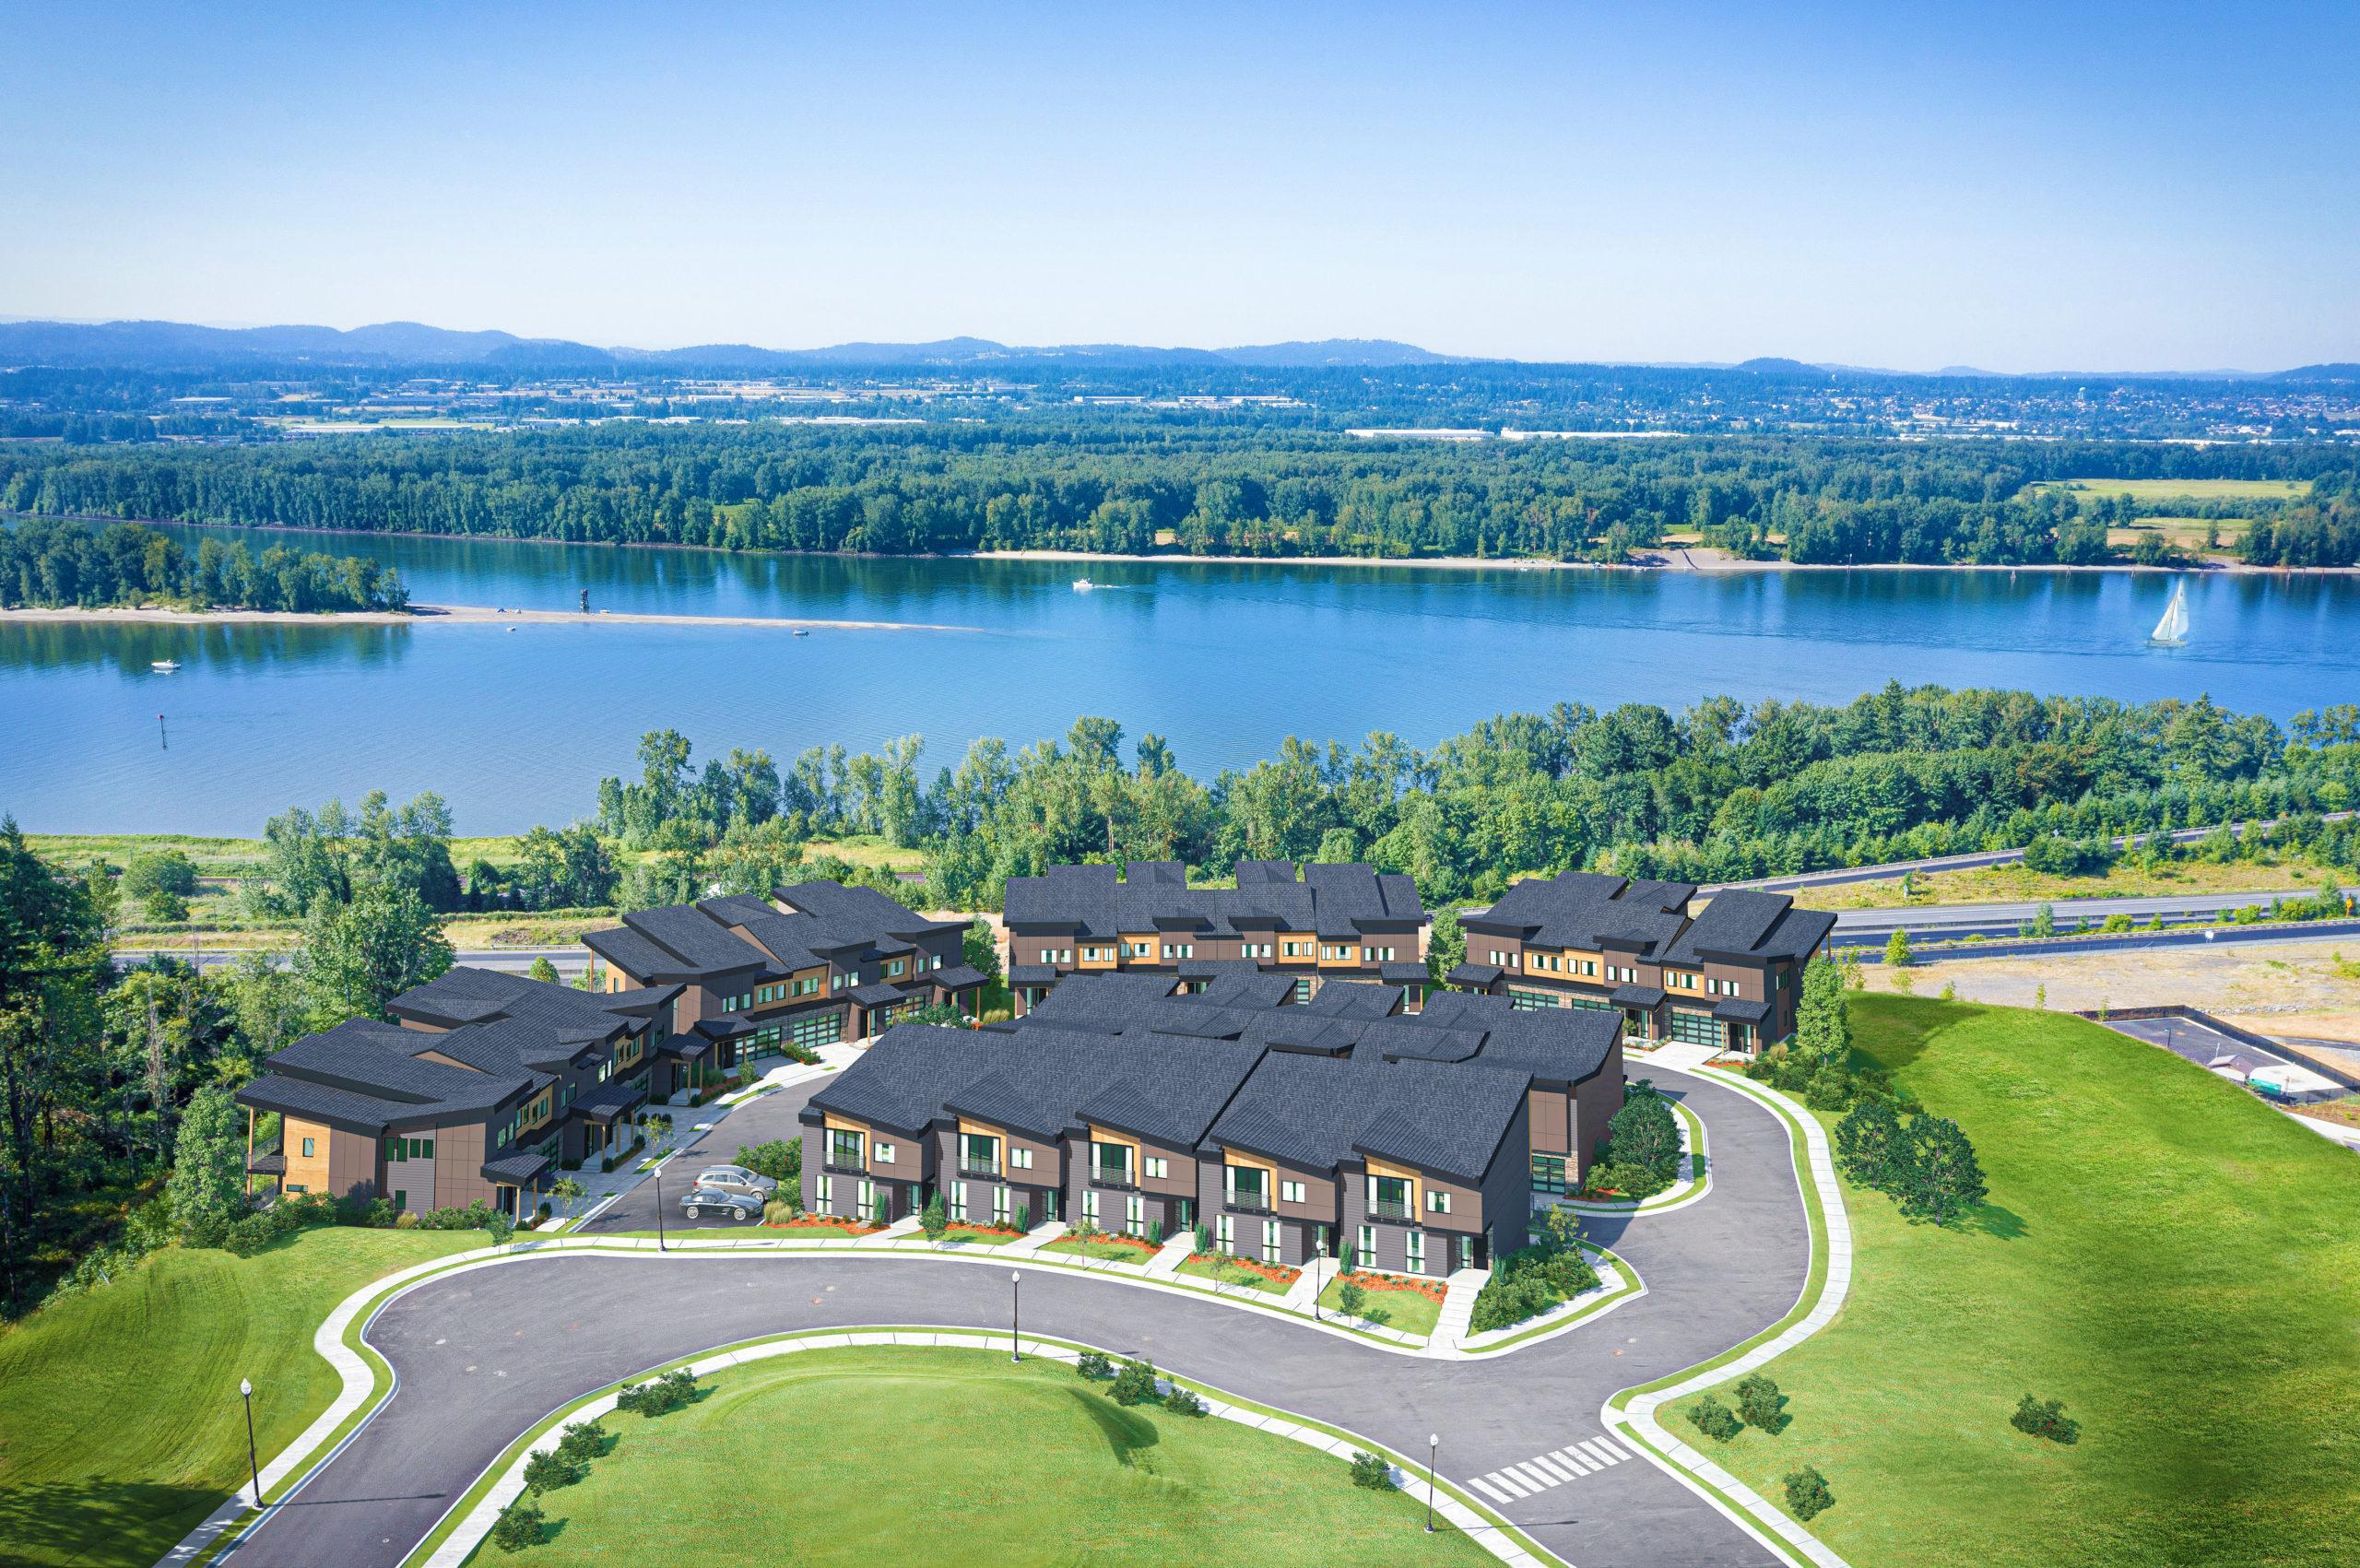
\includegraphics[width=\textwidth]{clark_county}
\end{figure}
\newpage

\tableofcontents
\newpage

\section{Introduction}
    Imagine you are preparing to search for your dream home in Clark County, Washington, and would 
    like to know how much that home is going to cost. You have the ability to specify the amount of 
    living space, acrage, the city, and the overall quality. The data mining task dicussed in this 
    report will see this idea through, and discover how to make accuate predictions on homes sold in 
    in Clark County.

    The purpose of this project is to tailor machine learning models to enable the ability to make 
    accurate house price predictions for Clark County in Washington State. 
    With housing prices rising consistenly in recent years, it could be useful to have a 
    prediction model that can guess at the pricing of a home based on various 
    criteria. This project will address this specific use case, and analyze the use of a number of 
    different models to determine which model produces most precise predictions.

    This report will also give an overview of all components of the methodology used to implement housing 
    price prediction. The data \cite{cc_data} used in this project was found on the Clark County government website
    which provides us with details on residential property sales for the year of 2021. 

\section{Data Mining Task}
    The data mining task involes using real-world data to make a prediction based on various features. 
    Analyzing the use of three different machine learning models will yield for better decision making 
    in terms of what model performs best on predicting housing prices based on various criteria. The models
    will all train and test on the same data, and will all be evaluated and validated using the same parameters. 
    The three models being used are: linear regression, decision tree, and random forest. 

    A number of different variables exist when approaching this data mining task. Ideally, the machine learning model 
    will use as many features as possible to generate more accurate predictions. The more specific the criteria 
    of the homes, the better the yielded results. During the data cleaning process, there will be data which is excluded 
    from the original data set. Some data is not easily processed by a machine learning model and therefore
    will be either excluded or modified in order to yield the best results. 

    The main goal of this project is to implement different machine learning models on housing data and perform anaysis on the results 
    to see which performs the best.

\section{Methodology}
    \subsection{Gathering Data}
    The data that is used for this project came from the Clark County website\cite{cc_data}. This site holds records from previous
    years regarding residential home purchases. Luckily, the data for homes purchased in 2021 came in the form of a csv file which makes it easier to work with. 
    This dataset was especially useful to make home pricing predictions because it provided a decent number of different attributes 
    to each home which was sold. Additionally, there are nearly 10,000 rows of data to use which helps bolster the training and testing 
    results. Statistically, more data helps produce better predictions with higher precision.

    Initially, the dataset came with columns of information regarding the address, rated quality, build year, as well as 
    acrage and square footage of living space. These are all useful pieces of information to use in the machine learning process 
    since many similarly priced homes have similar attributes. Several of the data columns contained in this dataset will need to be 
    transformed from a categorical to a numerical representation. Thankfully, there are Python libraries designed to aid with the 
    data cleaning and pre-processing which is dicussed in the next several sections. 

    \subsection{Libraries and Modules}
    The technical methodology truly begins with utilizing Python libraries that are best suited for cleaning, 
    splitting, training, and testing the data. Popular data handling libraries such as Pandas and Numpy will be used. 
    Most of the machine learning work will be done using a variety of modules from the Sklearn, also known as Sci-Kit Learn, library. Within Sklearn, we can 
    use existing tools to help execute the data pre-processing, as well as both the training and testing. Sklearn has a variety
    of machine learning methods, from which we will be using ``LinearRegression", ``DecisionTreeRegressor", and ``RandomForestRegressor".

    Data-preprocessing tools like ``OneHotEncoder" are utilized to help with modifying categorical data. Machine learning models requrire
    numerical input, so this is one way to ensure that we can use categorical data properly. One hot encoding is a technique which allows 
    for a unique binary value to be a assigned to a category. This method is used often instead of merely assigning a category to a random 
    number. We do this because the training models typically interpret raw values differently and this may have an affect on the accuracy of 
    the resultant predictions\cite{onehot}.

    \begin{figure}[H]
        \centering
        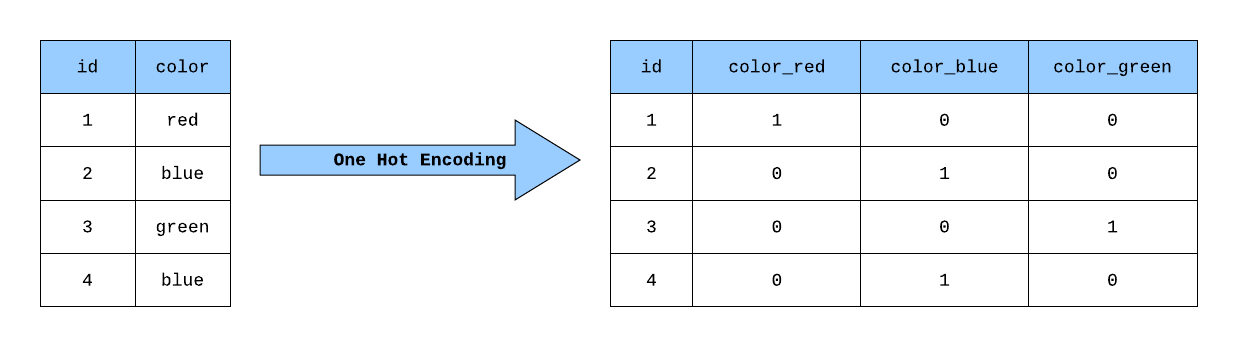
\includegraphics[width=\textwidth]{one_hot_encoding}
        \caption{Example of one hot encoding\cite{onehot2}}
    \end{figure}

    ``StandardScaler" is another data pre-processing tool which is used to standardize the dataset before it is used in training 
    and testing. Essentially, the data is normalized because the machine learning model may behave in unexpected ways as much of the 
    statistics used in these models relies on a standard (Gaussian) normal distribution\cite{sscaler}.
    
    \subsection{Cleaning Data}
    One of the most important phases in this data mining task is to clean and process the data properly. 
    In order to provide the machine learning model with the best input, several transformations need to be
    made to the inital dataframe containing the dataset. This process was the most time consuming, but also 
    made for a simple process when implementing each of the machine learning models.
    
        \subsubsection{Removing Unwanted Data}
        The first task in cleaning data is to remove data we do not need or want to include in the final dataframe 
        used to split for trainging and testing. For some reason, there was an exorbitant number of `Unnamed' columns
        in the original dataframe. Not only does this take up a lot of unneccessary space in memory, but it can have a negative 
        effect on the outcome of the prediction results. In addition to this, it was also neccessary to drop any rows with 
        null values in columns that would be included in the final dataframe. Thankfully, each row in the dataset had a 
        unique identifier, so there was no need to remove any duplicates from the set.

        Another instance of removing unwanted data is regarding outliers in the data which significantly impact the final 
        prediction results. The actual sale price of a home is one of the most important pieces of information to consider 
        during the process. After running the models on the cleaned data, it was clear that homes which were greater than \$500,000 
        had a higher margin of error than those which were priced under \$500,000. 
        
        This brought on the idea of filtering the data to include all home prices which were less than \$500,000. As a result, the housing price predictions saw a much 
        smaller margin of error. In fact, the mean absolute error went down from 9\% to 7\%. The figures below compare the two 
        cases where there is a maximum threshold of \$500,000 homes and no threshold (left and right respectively). Note that the 
        figure with no pricing threshold is essentially a zoomed out version of the figure with a threshold. Ultimately, it would 
        be important to include a feature where someone can specify a price range in their home attribute criteria to produce 
        more accurate results.
        \begin{figure}[H]
            \begin{subfigure}{0.5\textwidth}
                \centering
                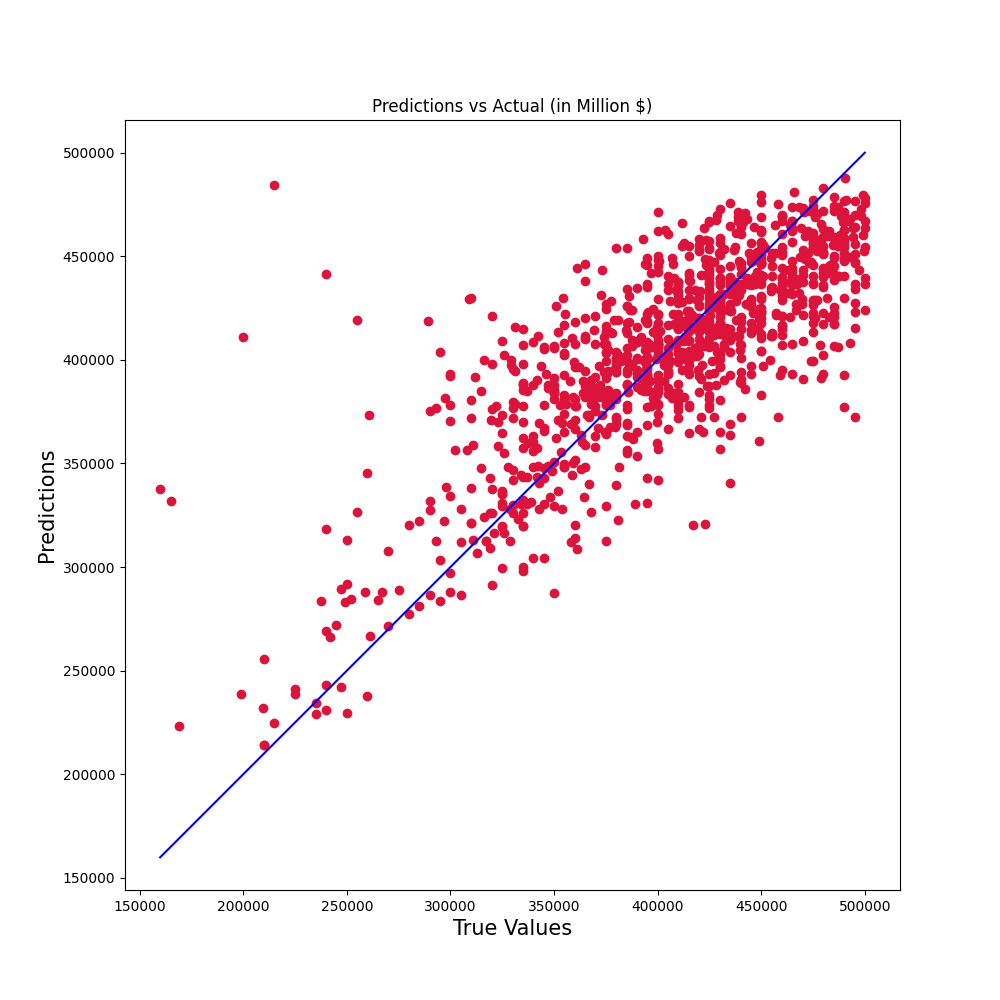
\includegraphics[width=\textwidth]{500limit}
            \end{subfigure}
            \hfill
            \begin{subfigure}{0.5\textwidth}
                \centering
                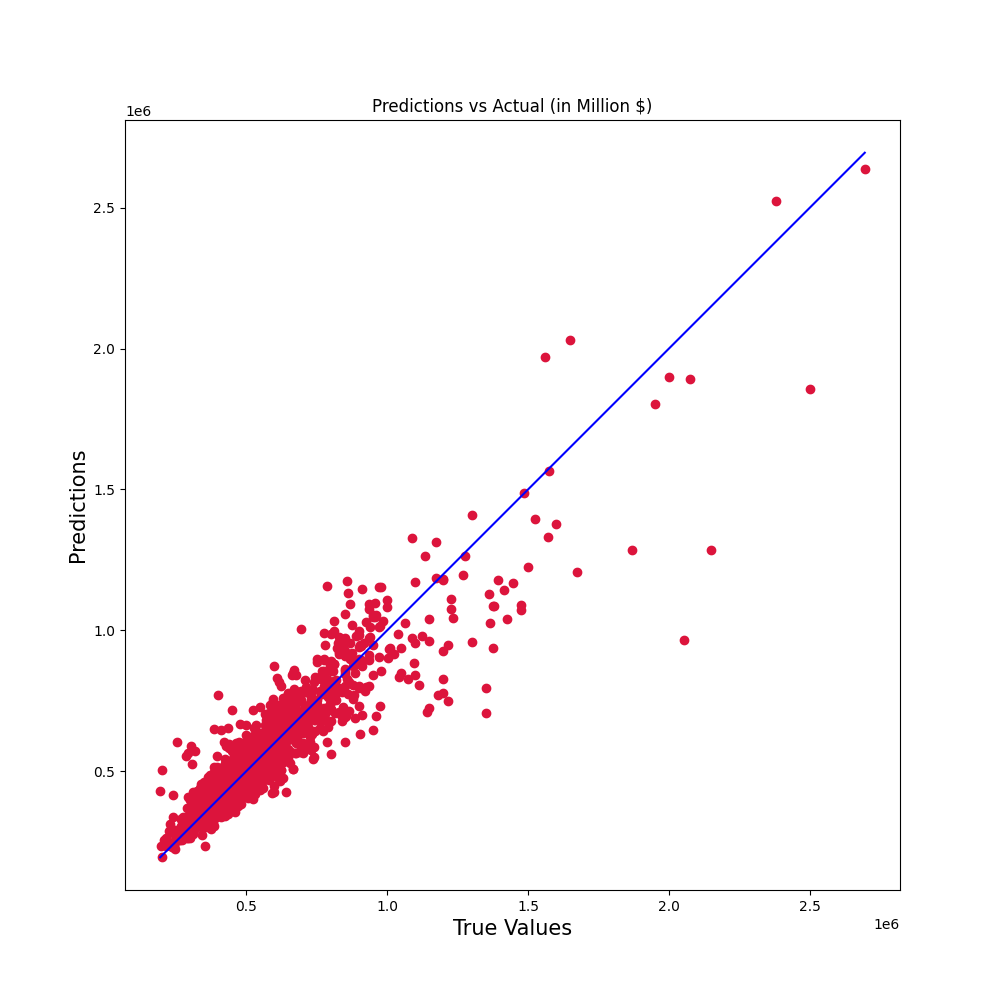
\includegraphics[width=\textwidth]{no_thresh}
            \end{subfigure}
            \caption{Difference in implementing a home price threshold}
        \end{figure}

        \subsubsection{Categorical vs. Numerical Data}
        A common issue when cleaning data for a machine learning application is the desire to include categorical data. In order for 
        some machine learning models to work properly, it needs to recieve an input of numerial data. This is exactly the case with 
        the regression models that are used in this project. Transforming categorical data to numerical can be simplified with the use 
        of one hot encoding. 
        
        Essentially, one hot encoding will transform each unique category into a new column in the dataframe. Then 
        it assigns a binary value (0 for no, 1 for yes) which indicates whether the row falls in that category. This is preferred over 
        simply renaming the categories to a new values because some machine learning models might treat numerical values differently.

        The two columns which were categorical and had a major impact on the learning predictions were `STYLE' and `Parcel Address'. The 
        `STYLE' column specified whether the home had one or two stories, was a ranch style home, or split level. The `Parcel Address' 
        originally specified the street address of the property. Instead of using the entire address string, I decided to extract the city 
        from which the property was in. This was a factor which also could have an influence on the home price since areas like Camas differ 
        than those in Battle Ground. 

        \subsubsection{Organization}
        The last step in completing the cleaning process was to ensure that the feature we desire to predict was the last column in the 
        dataframe. This was a simple transformation where the `ORIGINAL SALE AMOUNT' was popped from the dataframe, and immediately inserted 
        as the last column. This helps during the phase of splitting our data into the training and testing set since it will make it simple to 
        refer to that attribute later during prediction time.

    \subsection{Splitting Train and Test Set}
        \subsubsection{Splitting the Sets}
        When splitting the data into training and testing sets, it is important to keep in mind what attribute we are attempting to predict. 
        In this case, the housing price is being predicted based on other attributes of the home. During the splitting phase, we utilize a method
        from the model\_selection module in Sci-Kit Learn called `train\_test\_split'. This method requires a matrix and a vector. The matrix contains 
        the independent variables and the vector contains the dependent variables (responses). 
        
        We also specify the ratio of test set we desire which 
        is 20\%. The is a standard ratio that is used in supervised learning. Another setting is the `random\_state', which we 
        will be setting to 0. The random state variable controls the shuffling of the data before applying the split\cite{train_test_split}. By setting it to 0, we will see 
        consistent results which helps when analyzing prediction results and making optimizations.

        After supplying the method with this information, it will return a list which contains train-test split of inputs. This allows us to proceed with 
        the next and final step in data pre-processing.

        \subsubsection{Standardization}
        Using the `StandardScaler' method from the preprocessing module in the Sci-Kit Learn library, we can standardize features before training.
        The value in doing this helps improve the behavior of the machine learning estimators we use later on. This is a common requirement for many 
        models as the statistical methods used require the data to adhere to a Gaussian distribution. The independent variables in the training set will use the `fit\_transform' method 
        and the independent variables for the testing set will use `transform'. These differ as we only want to use a fitting method on the training dataset. The 
        next step is to implement different machine learning models.
    \subsection{Model Implementation}
    The models used in this project will be different types of regressors instead of classifiers. To highlight the difference between regression and classification, the following are the 
    definitions of the two concepts\cite{class_vs_reg}:
    \begin{itemize}
        \item \textbf{Regression}: The task of predicting a continuous quantity.
        \item \textbf{Classification}: The task of predicting a discrete class label or category.
    \end{itemize}
    Since the goal in mind here is to predict a numerical value, we will proceed with regression algorithms.
        \subsubsection{Linear Regression}
        The first model to be used for implementation is the well-known linear regression model. In statistics, linear regression is a linear approach 
        for modelling the relationship between an independant and dependant variable. This is a common method used in machine learning since we have the 
        ability to predict one value based on this linear relationship. 

        The linear regression estimator is the function which will be continuously adapted during training. The equation will be that of the form: $y = mx + b$.
        When working with linear regression, the main goal is to find a line of best fit according to the independent and dependant variable data provided. The 
        mean squared error is used as the cost function:
        \begin{center}
            \Large \fbox{$MSE = \frac{1} {N} \sum_{i = 1}^{n}(y_i - (a_1 x_i + a_0))^2$}
        \end{center}
        \normalsize

        The implementation is quite simple. Since most of the hard work was completed during the cleaning and pre-processing phases, we can plug 
        and play. Using the `LinearRegression' class from the `linear\_model' module in Sci-Kit Learn, we simply fit the training data to the model, and 
        make a prediction on the test data. 

        \renewcommand{\baselinestretch}{1.5}
        \begin{lstlisting}[language=Python, caption=Linear regression implementation]
    def linear_reg_learner(x_train, x_test, y_train, y_test):
        # Training Linear Regression model on training set
        print("Training...")
        model_LR = LinearRegression()
        model_LR.fit(x_train, y_train)
        # Predicting test set results
        print("Testing...")
        y_pred = model_LR.predict(x_test)
        return (y_pred, y_test)
        \end{lstlisting}
        \renewcommand{\baselinestretch}{2}

        \subsubsection{Decision Tree}
        The next model implementation uses a decision tree algorithm. The basic idea behind decision trees is that they have a flowchart-like structure. 
        Each node in the flowchart (tree) represents a feature, and each branch represents a decision rule. The tree is traversed recusively until data finds 
        its home in a node leaf of best fit. This is a great way to describe non-linear data, so it gives us a chance to observe whether the data has either a 
        linear or non-linear relationship. Below is a figure that illustrates the decision tree structure.

        \begin{figure}[H]
            \centering
            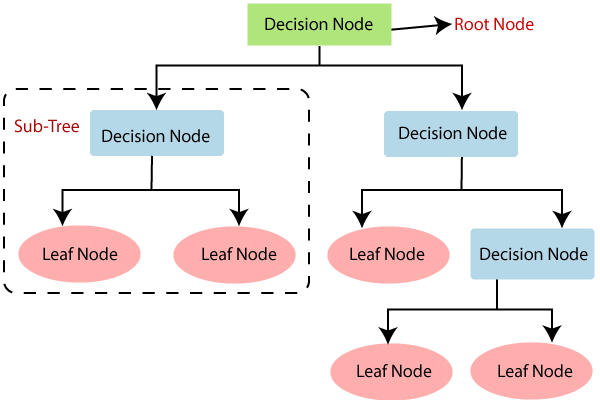
\includegraphics[width =0.8\textwidth]{d_tree}
            \caption{Decision tree structure}
        \end{figure}

        Implementation of this model is similar to the linear regression implementation. Using the `DecisionTreeRegressor' class from the `tree' module available 
        in Ski-Kit Learn, we fit the data to the regressor. We also set the `random\_state' parameter equal to 0 in order to maintain consistency in our results. 
        Then we can proceed with predictions.

        \renewcommand{\baselinestretch}{1.5}
        \begin{lstlisting}[language=Python, caption=Linear regression implementation]
    def decision_tree_learner(x_train, x_test, y_train, y_test):    
        # Training Decision Tree Regression model on training set
        print("Training...")
        classifier = DecisionTreeRegressor(random_state = 0)
        classifier.fit(x_train, y_train)
        # Predicting test set results
        print("Testing...")
        y_pred = classifier.predict(x_test)
        return(y_pred, y_test)
        \end{lstlisting}
        \renewcommand{\baselinestretch}{2}

        \subsubsection{Random Forest}
        The final machine learning model implementation uses a random forest technique. This is also a model which is best suited for 
        non-linear data or complex relationships between features and labels. It is the optimal model to use when linear models are overfitting.
        While non-linear, decision trees are also prone to overfitting, especially when we don't provide the model with a maximum depth.
        To mitigate this, random forests use a collection of decision trees in order to make predictions. This technique classifies as an ensemble model.
        Random forests also use a bagging method which is used to reduce variance in a noisy dataset. Given that this is real-world data, and as we have seen 
        in the cleaning phase, the data is quite noisy. 

        The implementation of a random forest uses the `RandomForestRegressor' class from the `ensemble' module in Sci-Kit Learn. The criterion for this 
        usage will be `squared\_error' which is set by default. The `random\_state' parameter is also set to 0 to maintain our results.

        \renewcommand{\baselinestretch}{1.5}
        \begin{lstlisting}[language=Python, caption=Linear regression implementation]
    def random_forest_learner(x_train, x_test, y_train, y_test):
        # Training Random Forest model on training set
        print("Training...")
        classifier = RandomForestRegressor(random_state = 0)
        classifier.fit(x_train, y_train)
        # Predicting test set results
        print("Testing...")
        y_pred = classifier.predict(x_test)
        return (y_pred, y_test)
        \end{lstlisting}
        \renewcommand{\baselinestretch}{2}

    \subsection{Analysis and Evaluation}
    To analyze the prediction results from all three machine learning models, I attempted to implement a confusion 
    matrix which is a common metric for machine learning analysis. However, since we are not evaluating a discrete 
    value, the confusion matrix will not yield any useful information. Instead, using the `mean\_absolute\_percentage\_error'
    method gave a better idea of the accuracy in the predictions. Alongside the mean absolute error, I decided to 
    calculate how many occurances the model predicted under or over the actual home price as well as the average amount 
    predicted under or over. A visualization of the correlation between predicted and actual value is also produced 
    upon program execution.

        \subsubsection{Linear Regression}
        The linear regression model yielded a mean absolute error of ~14.7\% when no threshold on home price range is specified. 
        When there is a upper limit of \$500,000 for home prices, the error reduces to ~10.4\%. Additionally, the housing price 
        predictions were $\pm$\$75,000 from the actual value with no threshold on average. When a threshold is introduced, the predictions 
        averaged at $\pm$\$40,000 from the actual value. 

        The analysis also shows that when a threshold is introduced, the model tends to predict under the actual value more often.
        The opposite it true when there is no threshold present. This makes sense due to the outliers having an effect on the data 
        points being examined. Below are two visual which show the difference between results correlation with a threshold, and without
        (left and right respectively).

        \graphicspath{ {/home/amskyepi/Documents/Fall2022/CS315/Final_Project/Visuals} }
        \begin{figure}[H]
            \begin{subfigure}{0.5\textwidth}
                \centering
                \includegraphics[width=\textwidth]{With_Threshold/linear_reg_results}
            \end{subfigure}
            \hfill
            \begin{subfigure}{0.5\textwidth}
                \centering
                \includegraphics[width=\textwidth]{No_Threshold/linear_reg_results}
            \end{subfigure}
            \caption{Difference in linear regression predictions when introducing a threshold}
        \end{figure}

        The graphs show that there is a decent amount of clustering near the line $y = x$. The optimal outcome is that as many points fit 
        that line as possible because it means our predictions are usually accurate. The reason I implemented a threshold with the home pricing
        in the first place is because I noticed how the data points clustered towards the bottom of the line in the figure to the right. The figure 
        on the left shows a little less clustering, however the prediction results tend to be higher in accuracy. I hypothesize that if I were to 
        narrow the home price range even closer, the prediction accuracy would continue to improve. 

        \subsubsection{Decision Tree}
        Using the decision tree, the accuracy improved when comparing to the linear regression model used previously. When no threshold was 
        implemented, the model produced a mean absolute error of ~12.3\% and predictions that were $\pm$\$70,000 from the actual home price. 
        When a threshold was introduced, the error reduced to ~9.5\% and predictions were $\pm$\$35,000 from the actual value. 
        
        Interestingly enough, with or without a threshold, the model tends to over predict the home price. This is a result of overfitting, which was mentioned when 
        discussing the differences in machine learning models. Decision trees which do not specify a maximum depth tend to overfit, which is exactly 
        what happened. The figures below illustrate the difference between implementing a price threshold and having no threshold (left and right respectively).

        \begin{figure}[H]
            \begin{subfigure}{0.5\textwidth}
                \centering
                \includegraphics[width=\textwidth]{With_Threshold/decision_tree_results}
            \end{subfigure}
            \hfill
            \begin{subfigure}{0.5\textwidth}
                \centering
                \includegraphics[width=\textwidth]{No_Threshold/decision_tree_results}
            \end{subfigure}
            \caption{Difference in decision tree predictions when introducing a threshold}
        \end{figure}

        Notice that in the left figure, the data points are less clustered. I would like to see what happens when a maximum depth is introduced. 
        I would imagine that when a maximum depth is introduced, the data points would fit the line $y = x$ more closely. 

        Another intersting observation is the difference between the graphs for a linear regression model and decision tree model when 
        no price threshold is included. The decision tree is able to predict the higher priced homes a bit closely than linear regression.

        \subsubsection{Random Forest}
        The random forest results are even better than the decision tree. When no threshold was implemented, the mean absolute error 
        was ~9.4\% which is about the same performance as the decision tree with a threshold. Even better, when a threshold was inclulded 
        the error reduced to ~7.3\%. This turned out to be the best results when doing basic implementations of all models. 

        When no threshold was included, the predictions were $\pm$\$55,000. On the other hand, once a threshold was introduced, the predictions 
        were averaged at $\pm$\$30,000 which is slightly better results than the decision tree yielded. Below are figures that show how the 
        random forest performed with a threshold vs without (left and right respectively).

        \begin{figure}[H]
            \begin{subfigure}{0.5\textwidth}
                \centering
                \includegraphics[width=\textwidth]{With_Threshold/random_forest_results}
            \end{subfigure}
            \hfill
            \begin{subfigure}{0.5\textwidth}
                \centering
                \includegraphics[width=\textwidth]{No_Threshold/random_forest_results}
            \end{subfigure}
            \caption{Difference in random forest predictions when introducing a threshold}
        \end{figure}

        For either threshold or no, the random forest produced better results and a better correlation between the prediction and actual 
        value. Notice how the data points are slightly more grouped towards the line $y = x$ compared to the other models. Using these visuals 
        significantly helped to get a difference perspective on how the models performed when making predictions.

\section{Conclusion}
During analysis, I conclude that the best scenario that was tested was implementing a random forest algorithm with a price threshold included. 
The threshold that I decided on was a range of [0, 500000]. This is due to prior analysis of the data points on the graph with all prices included.
Most of the home prices were \$500,000 or less. This means that I would be eliminating a minimal amount of outliers, but also making a significant 
positive impact on the prediction accuracy. 

One problem when including a price range is that it limits the pricing predictions. Essentially, a home that would be estimated at \$500,000 or higher would 
be eliminated as a possibility. One way that this could be implemented more smoothly in practice 
would be to allow the user to specify a desired price range (both a minimum and maximum). This way, the algorithm could easily filter out homes that are not in that 
range, and tailor a model that fits their needs. This feature is in addition to any other home attributes they would like to specify (style, area, acrage).

Another interesting finding is how the decision tree appeared to overfit the predictions. I think with some tuning to the parameters of the decision 
tree method, the performance would improve. 

Overall, I am happy with the results of the random forest. It produced an accuracy of about 93\% when a threshold was implemented. This project was simply a baseline 
usage of the random forest, and could be improved upon by adjusting the hyperparameters and testing out different machine learning algorithms. 

\newpage
\begin{thebibliography}{6}
    \bibitem{cc_data}
    Clark County Washington \url{clark.wa.gov/assessor/residential-property-sales-information},
    Accessed 8 Dec 2022

    \bibitem{onehot}
    Sci-Kit Learn Documentation \url{https://scikit-learn.org/stable/modules/generated/sklearn.preprocessing.OneHotEncoder.html},
    Accessed 9 Dec 2022

    \bibitem{sscaler}
    Sci-Kit Learn Documentation \url{scikit-learn.org/stable/modules/generated/sklearn.preprocessing.StandardScaler.html},
    Accessed 9 Dec 2022

    \bibitem{onehot2}
    Novak, George. `Building a One Hot Encoding Layer with Tensorflow' \url{https://towardsdatascience.com/building-a-one-hot-encoding-layer-with-tensorflow-f907d686bf39},
    Accessed 9 Dec 2022

    \bibitem{train_test_split}
    Sci-Kit Learn Documentation \url{https://scikit-learn.org/stable/modules/generated/sklearn.model_selection.train_test_split.html},
    Accessed 11 Dec 2022

    \bibitem{class_vs_reg}
    Brownlee, Jason. `Difference Between Classification and Regression in Machine Learning', 11 Dec 2017. \url{https://machinelearningmastery.com/classification-versus-regression-in-machine-learning/},
    Accessed 11 Dec 2022
\end{thebibliography}

\end{document}